%%% Local Variables: 
%%% mode: latex
%%% TeX-master: "courseml"
%%% End: 

%%%%%%%%%%% COLORS

\definecolor{darkgrey}{rgb}{0.2,0.2,0.2}
\definecolor{grey}{rgb}{0.9,0.9,0.9}
\definecolor{darkblue}{rgb}{0.0,0.0,0.5}
\definecolor{darkpurple}{rgb}{0.4,0.0,0.4}
\definecolor{darkred}{rgb}{0.5,0.0,0.0}
\definecolor{darkorange}{rgb}{0.5,0.45,0.4}
\definecolor{darkgreen}{rgb}{0.0,0.5,0.0}
\definecolor{darkergreen}{rgb}{0.0,0.4,0.0}
\definecolor{lightblue}{rgb}{0.8,0.8,1.0}
\definecolor{lightgreen}{rgb}{0.8,1.0,0.8}
\definecolor{lightred}{rgb}{1.0,0.8,0.8}
\definecolor{lightyellow}{rgb}{1.0,1.0,0.8}
\definecolor{lightorange}{rgb}{1.0,0.9,0.8}
\definecolor{lightgrey}{rgb}{0.96,0.97,0.98}
\definecolor{Sepia}{HTML}{671800}

%%%%%%%%%%%%% FORMATTING
%
%\newcommand*\chapterlabel{}
%\makeatletter
%\titleformat{\chapter}%
%  [block]                                % shape
%  {\gdef\chapterlabel{}
%   \normalfont\sffamily\Huge\bfseries\scshape}            % format applied to label+text
%  {\gdef\chapterlabel{\thechapter~|~}}    % 
%  {0pt}                                  % horizontal separation between label and title body
%  {\begin{tikzpicture}[remember picture,overlay]
%    \node[yshift=-3cm] at (current page.north west)
%      {\begin{tikzpicture}[remember picture, overlay]
%        \draw[fill=lightgreen] (0,0) rectangle
%          (\paperwidth,3cm);
%        \node[anchor=east,xshift=.9\paperwidth,rectangle,
%              rounded corners=20pt,inner sep=11pt,
%              fill=darkergreen]
%              {\color{white}\chapterlabel#1};
%       \end{tikzpicture}
%      };
%   \end{tikzpicture}
%  }% before the title body
%  []%after the title body
%\makeatother 
%%\titlespacing*{\chapter}{0pt}{50pt}{-10pt}
%
%\newcommand{\sectionsize}{}
%\titleformat{\section}%
%  [hang]% shape
%  {\normalfont\Large\itshape}% format applied to label+text
%  {\textcolor{darkergreen}{\makebox[0pt][r]{\thesection\quad }#1}}% label
%  {1em}% horizontal separation between label and title body
%  {}% before the title body
%  []% after the title body
%
%\titleformat{\subsection}%
%  [hang]% shape
%  {\normalfont\large\itshape}% format applied to label+text
%  {\textcolor{darkergreen}{\makebox[0pt][r]{\thesubsection\quad }#1}}% label
%  {1em}% horizontal separation between label and title body
%  {}% before the title body
%  []% after the title body



%%%%%%%%%%% EXERCISE STUFF

\newtheorem{Ex}{Exercise}
\newenvironment{exercises}{\section{Exercises}}{}
% \center\begin{tabular}{c}\hline{\bf\Large Exercises}\\\hline\end{tabular}}{}

%\Newassociation{solution}{Soln}{solutions}
%\Newassociation{hint}{Hint}{solutions}
\newcommand{\prehint}{~[Hint]}
\newcommand{\presolution}{}
\newcommand{\Opensolutionshook}[2]%
  {\Writetofile{#1}{}}
%\renewcommand{\Solnlabel}[1]{%
%  {\Large\linespread{1}%
%  \begin{tabular}{|p{\textwidth}@{}|}%
%    \hline%
%    \emph{Solution #1}\\%
%    \hline%
%  \end{tabular}\newline}}
%\renewcommand{\Hintlabel}[1]{\emph{Hint #1}}


\newcommand{\emptylist}{[ ]}
\newcommand{\pushlist}[1]{{\ensuremath \oplus} #1}

\newcommand*\learningproblemargument{}
\newsavebox{\learningproblembox}
\newenvironment{learningproblemenv}[1]
  {\gdef\learningproblemargument{#1}\begin{lrbox}{\learningproblembox}\begin{minipage}{4in}}
  {\end{minipage}\end{lrbox}%
   \tikzstyle{mybox} = [draw=darkgreen, fill=green!5, very thick, rectangle, rounded corners, inner sep=10pt, inner ysep=12pt]%
   \tikzstyle{fancytitle} =[fill=darkgreen, text=white, rectangle, rounded corners]%
   \vspace{1em}
   \noindent
   \begin{tikzpicture}
     \node [mybox] (box) {\usebox{\learningproblembox}};
     \node [fancytitle, right=10pt] at (box.north west) {\normalfont\sffamily\Large\bfseries\scshape Task: \learningproblemargument};
   \end{tikzpicture}
  }

\newcommand{\learningproblem}[3]{
  \begin{learningproblemenv}{#1}
    \emph{Given:}
    \begin{enumerate}
      #2
    \end{enumerate}
    \emph{Compute:} #3
  \end{learningproblemenv}}

\newcommand{\lprob}[1]{{\normalfont\sffamily\scshape #1}}

%%%%%%%%%%% ENVIRONMENTS

\DefineVerbatimEnvironment%
  {chapternotes}{Verbatim}
  {baselinestretch=1.0,frame=single,fillcolor=\color{lightgreen}}
%\renewenvironment{chapternotes}{\begin{comment}}{\end{comment}}

\newenvironment{editedout}{\begin{comment}}{\end{comment}}

\newenvironment{derivation}
  {\begin{eqnarray}}
  {\end{eqnarray}}

\newcommand{\derivstep}[2]{#1\sidenote{#2}}

%\makeatletter\newenvironment{learninggoals}{%
%   ~\\\noindent\begin{lrbox}{\@tempboxa}\begin{shadowblock}{\columnwidth}\begin{itemize}}{\end{itemize}\end{shadowblock}\end{lrbox}%
%   {\usebox{\@tempboxa}}
%}\makeatother

%\newenvironment{learningobjectives}
%  {\begin{marginfigure}\begin{learninggoals}\item[]\item[] \hspace{-2em} {\bf Learning Objectives:}}
%  {\end{learninggoals}\end{marginfigure}}

\newsavebox{\objectivesbox}
\newlength{\objectivesheight}
\newenvironment{learningobjectives}
  {\begin{lrbox}{\objectivesbox}\begin{minipage}{2in}\vspace{2pt}{\bf Learning Objectives:}\begin{footnotesize}\begin{itemize}}
  {\end{itemize}\end{footnotesize}\end{minipage}\end{lrbox}\begin{textblock}{2}(10.2,2.5)\begin{shadowblock}{2in}\usebox{\objectivesbox}\end{shadowblock}\end{textblock}\settoheight{\objectivesheight}{\usebox{\objectivesbox}}}

\newenvironment{chapterintro}
  {}
  {}

\newcommand*\vignetteargument{}
\newsavebox{\vignettebox}
\newenvironment{vignette}[1]
  {\gdef\vignetteargument{#1}\begin{lrbox}{\vignettebox}\begin{minipage}{6.4in}}
  {\end{minipage}\end{lrbox}%
   \tikzstyle{mybox} = [draw=Periwinkle, fill=Periwinkle!5, very thick, rectangle, rounded corners, inner sep=10pt, inner ysep=12pt]%
   \tikzstyle{fancytitle} =[fill=Periwinkle, text=white, rectangle, rounded corners]%
   \vspace{1em}
   \noindent
   \begin{tikzpicture}
     \node [mybox] (box) {\usebox{\vignettebox}};
     \node [fancytitle, right=10pt] at (box.north west) {\normalfont\sffamily\Large\bfseries\scshape Vignette: \vignetteargument};
   \end{tikzpicture}
  }

%[transform shape, baseline=-3.5cm]
\newcommand*\mathreviewargument{}
\newsavebox{\mathreviewbox}
\newenvironment{mathreview}[1]
  {\gdef\mathreviewargument{#1}\begin{lrbox}{\mathreviewbox}\begin{minipage}{6.4in}}
  {\end{minipage}\end{lrbox}%
   \tikzstyle{mybox} = [draw=Sepia, fill=Sepia!5, very thick, rectangle, rounded corners, inner sep=10pt, inner ysep=12pt]%
   \tikzstyle{fancytitle} =[fill=Sepia, text=white, rectangle, rounded corners]%
   \begin{figure*}[t]
     \begin{tikzpicture}
       \node [mybox] (box) {\usebox{\mathreviewbox}};
       \node [fancytitle, right=10pt] at (box.north west) {\normalfont\sffamily\Large\bfseries\scshape Math Review | \mathreviewargument};
     \end{tikzpicture}
     \caption[Math Review: \mathreviewargument]{~}
   \end{figure*}%
  }


%\newenvironment{chapterquote}
%  {\textblockcolor{grey}\begin{textblock}{6.5}(8,1)}
%  {\end{textblock}}

%\newenvironment{chapterimage}
%  {\textblockcolor{white}\begin{textblock}{6.5}(8,1)}
%  {\end{textblock}}


%  {\par\linespread{1}\center%
%   \begin{greybox}%
%   \begin{tabular}{|p{4in}|}%
%     \hline\vspace{+0.02in}%
%     \rule{1ex}{1ex} Learning Goals \rule{1ex}{1ex}%
%     }
%  { \vspace{+0.05in}\\\hline%
%   \end{tabular}\vspace{+0.1in}\end{greybox}\\}\makeatother


%%%%%%%%%%% COMMANDS

\newcommand{\bigemph}[1]{\textcolor{darkblue}{\bf #1}}

\newcommand{\dependencies}[1]{\marginnote[2.5in]{Dependencies: #1}}

%\newcommand{\dependencies}[1]{\begin{textblock}{2}(10.2,2.5)Dependencies: #1\end{textblock}}

%\sethlcolor{lightyellow}

\newcommand{\concept}[1]{\hl{\bf #1}\index{#1}}
\newcommand{\koncept}[2]{\hl{\bf #1}\index{#2}}

\newcommand{\chref}[1]{Chapter~\ref{#1}}


\newcommand{\chapterquote}[2]
  {\tikzstyle{mybox} = [draw=darkergreen, fill=green!20, very thick, rectangle, rounded corners, inner sep=5pt, inner ysep=5pt]
   \tikzstyle{fancytitle} =[fill=darkergreen, text=white]
   \begin{textblock}{7.5}(2,2.5)
   \begin{tikzpicture}[transform shape, rotate=0, baseline=-3.5cm]
   \noindent%
   \node [mybox] (box) {%
    \begin{minipage}[t!]{\textwidth}
      \noindent%
      \begin{large}%
      \textsf{#1}%
      \end{large}
      \hfill\textcolor{darkergreen}{\textsf{--~#2}}
    \end{minipage}
    };
%   \node[fancytitle] at (box.south) {\emph{-- #2}};
  \end{tikzpicture}
  \end{textblock}}

\newcommand{\chapterimage}[2]
  {\tikzstyle{mybox} = [draw=darkergreen, fill=green!20, very thick, rectangle, rounded corners, inner sep=5pt, inner ysep=5pt]
   \tikzstyle{fancytitle} =[fill=darkergreen, text=white]
   \begin{textblock}{7.5}(2,2.5)
   \begin{tikzpicture}[transform shape, rotate=0, baseline=-3.5cm]
   \noindent
   \node [mybox] (box) {%
    \begin{minipage}[t!]{\textwidth}
      \includegraphics[width=\textwidth]{#1}

      \hfill\textcolor{darkergreen}{\textsf{--~#2}}
    \end{minipage}
    };
%   \node[fancytitle] at (box.south) {\emph{-- #2}};
  \end{tikzpicture}
  \end{textblock}}

\newcommand{\chapterimageopt}[3]
  {\tikzstyle{mybox} = [draw=darkergreen, fill=green!20, very thick, rectangle, rounded corners, inner sep=5pt, inner ysep=5pt]
   \tikzstyle{fancytitle} =[fill=darkergreen, text=white]
   \begin{textblock}{7.5}(2,2.5)
   \begin{tikzpicture}[transform shape, rotate=0, baseline=-3.5cm]
   \noindent
   \node [mybox] (box) {%
    \begin{minipage}[t!]{\textwidth}
      \includegraphics[#2]{#1}

      \hfill\textcolor{darkergreen}{\textsf{--~#3}}
    \end{minipage}
    };
%   \node[fancytitle] at (box.south) {\emph{-- #2}};
  \end{tikzpicture}
  \end{textblock}}


\newcommand{\monthyear}{%
  \ifcase\month\or January\or February\or March\or April\or May\or June\or
  July\or August\or September\or October\or November\or
  December\fi\space\number\year
}

\newcommand{\blankpage}{\newpage\hbox{}\thispagestyle{empty}\newpage}
\newcommand{\mycite}[1]{\ e{\citealt{#1}}}
\newcommand{\bookurl}{\url{http://hal3.name/courseml/}}

\newcommand{\TODOFigure}[2]{%
  \begin{marginfigure}
    \framebox[\textwidth][c]{\begin{minipage}{\textwidth}\rule{0pt}{2in}\end{minipage}}
    \caption{{\tt #1}: #2}
    \label{fig:#1}
  \end{marginfigure}}

\newlength{\NextFigureOffset}
\newcommand{\ResetNextFigure}{\setlength{\NextFigureOffset}{0mm}}
\newcommand{\MoveNextFigure}[1]{\setlength{\NextFigureOffset}{#1}}

\ResetNextFigure{}

\newcommand{\Figure}[2]{%
  \begin{marginfigure}[\NextFigureOffset]
    \begin{centering}
    \includegraphics[width=\textwidth]{figs/#1}
    \caption{#2}
    \label{fig:#1}
    \end{centering}
  \end{marginfigure}
  \ResetNextFigure{}
  }

\newcommand{\Table}[4]{%
  \begin{margintable}
    \begin{centering}
    \begin{tabular}{#3}
      #4
    \end{tabular}
    \caption{#2}
    \label{tab:#1}
    \end{centering}
  \end{margintable}}

\newcommand{\TableSize}[5]{%
  \begin{margintable}
    \begin{centering}
    \begin{#1}
    \begin{tabular}{#4}
      #5
    \end{tabular}
    \caption{#3}
    \label{tab:#2}
    \end{#1}
    \end{centering}
  \end{margintable}}

\newcommand{\thinkaboutit}[1]{%
\marginnote{
   \noindent
  \begin{tikzpicture}[transform shape, rotate=0, baseline=-3.5cm]
   \node [draw=Blue, fill=Blue!10, very thick, rectangle, rounded corners, inner sep=8pt, inner ysep=5pt] (box) {%
    \begin{minipage}[t!]{1.8in}
      #1
    \end{minipage}
    };
   \node[fill=Blue, text=white] at (box.west) {\textsf{\LARGE ?}};
  \end{tikzpicture}
}
}

\newenvironment{myproof}[1]%
  {\begin{proof}[Proof of Theorem~#1]}
  {\end{proof}}

\definecolor{gray0.00}{rgb}{1,1,1}
\definecolor{gray0.20}{rgb}{0.9,0.9,0.9}
\definecolor{gray0.26}{rgb}{0.87,0.87,0.87}
\definecolor{gray0.30}{rgb}{0.85,0.85,0.85}
\definecolor{gray0.32}{rgb}{0.84,0.84,0.84}
\definecolor{gray0.33}{rgb}{0.835,0.835,0.835}
\definecolor{gray0.40}{rgb}{0.8,0.8,0.8}
\definecolor{gray0.48}{rgb}{0.76,0.76,0.76}
\definecolor{gray0.53}{rgb}{0.735,0.735,0.735}
\definecolor{gray0.57}{rgb}{0.715,0.715,0.715}
\definecolor{gray0.60}{rgb}{0.7,0.7,0.7}
\definecolor{gray0.68}{rgb}{0.66,0.66,0.66}
\definecolor{gray0.74}{rgb}{0.63,0.63,0.63}
\definecolor{gray0.80}{rgb}{0.6,0.6,0.6}
\definecolor{gray0.88}{rgb}{0.56,0.56,0.56}
\definecolor{gray1.00}{rgb}{0.5,0.5,0.5}
\newcommand{\showfscore}[1]{\cellcolor{gray#1}{#1}}

\renewcommand{\vx}{{\vec x}}
\renewcommand{\vw}{{\vec w}}
\renewcommand{\vg}{{\vec g}}
\renewcommand{\vz}{{\vec z}}
\renewcommand{\vth}{{\vec \theta}}
\renewcommand{\dotp}[2]{#1 \cdot #2}

\renewcommand{\txtif}{\text{if } }

\renewcommand{\ones}{\ensuremath{\mathbf{1}}}
\renewcommand{\zeros}{\ensuremath{\mathbf{0}}}
\renewcommand{\eye}{\ensuremath{\mathbf{I}}}

%\let\Oldtimes\times
%\renewcommand{\times}{\!\!\Oldtimes\!\!}

\renewcommand{\myiff}{\Longleftrightarrow}

\renewcommand{\subgrad}{\pmb\partial}

\renewcommand{\partialby}[1]{\frac \partial {\partial #1}}
\renewcommand{\partialof}[2]{\frac {\partial #1} {\partial #2}}

\renewcommand{\xth}[1]{{}^{\textcolor{darkgrey}{\textsf{(#1)}}}}
\renewcommand{\kth}{\xth{k}}
\renewcommand{\Kth}{\xth{K}}
\renewcommand{\kpth}{\xth{k-1}}
\renewcommand{\zth}{\xth{0}}
\renewcommand{\oth}{\xth{1}}
\newcommand{\newth}{\xth{new}}

\renewcommand{\pth}{p_{\vec\th}}

\newcommand{\becauseof}[1]{&&& \textsf{\textcolor{darkred}{#1}}}

% ALGORITHMIC STUFF

\algsetup{linenosize=\tiny,
          linenodelimiter=:
          }

\renewcommand{\algorithmicfont}{\normalfont\sffamily\normalsize\bfseries}
\newcommand{\algorithmiccolor}{darkpurple}

\newcommand{\GOTO}[1]{\STATE
  \textcolor{\algorithmiccolor}{\algorithmicfont goto~} {\large #1}}

\renewcommand{\algorithmicif}{\textcolor{\algorithmiccolor}{\algorithmicfont if}}
\renewcommand{\algorithmicrequire}{\textcolor{\algorithmiccolor}{\algorithmicfont Require:}}
\renewcommand{\algorithmicensure}{\textcolor{\algorithmiccolor}{\algorithmicfont Ensure:}}
\renewcommand{\algorithmicend}{\textcolor{\algorithmiccolor}{\algorithmicfont end}}
\renewcommand{\algorithmicif}{\textcolor{\algorithmiccolor}{\algorithmicfont if}}
\renewcommand{\algorithmicthen}{\textcolor{\algorithmiccolor}{\algorithmicfont then}}
\renewcommand{\algorithmicelse}{\textcolor{\algorithmiccolor}{\algorithmicfont else}}
\renewcommand{\algorithmicelsif}{\algorithmicelse\ \algorithmicif}
\renewcommand{\algorithmicendif}{\algorithmicend\ \algorithmicif}
\renewcommand{\algorithmicfor}{\textcolor{\algorithmiccolor}{\algorithmicfont for}}
\renewcommand{\algorithmicforall}{\textcolor{\algorithmiccolor}{\algorithmicfont for all}}
\renewcommand{\algorithmicdo}{\textcolor{\algorithmiccolor}{\algorithmicfont do}}
\renewcommand{\algorithmicto}{\textcolor{\algorithmiccolor}{\algorithmicfont to}}
\renewcommand{\algorithmicendfor}{\algorithmicend\ \algorithmicfor}
\renewcommand{\algorithmicwhile}{\textcolor{\algorithmiccolor}{\algorithmicfont while}}
\renewcommand{\algorithmicendwhile}{\algorithmicend\ \algorithmicwhile}
\renewcommand{\algorithmicloop}{\textcolor{\algorithmiccolor}{\algorithmicfont loop}}
\renewcommand{\algorithmicendloop}{\algorithmicend\ \algorithmicloop}
\renewcommand{\algorithmicrepeat}{\textcolor{\algorithmiccolor}{\algorithmicfont repeat}}
\renewcommand{\algorithmicuntil}{\textcolor{\algorithmiccolor}{\algorithmicfont until}}
\renewcommand{\algorithmicprint}{\textcolor{\algorithmiccolor}{\algorithmicfont print}}
\renewcommand{\algorithmicreturn}{\textcolor{\algorithmiccolor}{\algorithmicfont return}}
\renewcommand{\algorithmictrue}{\textcolor{\algorithmiccolor}{\algorithmicfont true}}
\renewcommand{\algorithmicfalse}{\textcolor{\algorithmiccolor}{\algorithmicfont false}}
\renewcommand{\algorithmicand}{\textcolor{\algorithmiccolor}{\algorithmicfont and}}
\renewcommand{\algorithmicor}{\textcolor{\algorithmiccolor}{\algorithmicfont or}}

\renewcommand{\algorithmiccomment}[1]{\hfill\textcolor{Sepia}{\normalfont\sffamily// #1}}

\newcommand{\VAR}[1]{\textcolor{darkblue}{\textit{#1}}}
\newcommand{\CON}[1]{\textcolor{darkgrey}{\textit{#1}}}
\newcommand{\FUN}[1]{\textcolor{blue}{\textsc{#1}}}
\newcommand{\STR}[1]{\textcolor{darkergreen}{\textsc{#1}}}
\newcommand{\VARm}[1]{\textcolor{darkblue}{\ensuremath #1}}
\newcommand{\FUNm}[1]{\textcolor{blue}{\ensuremath #1}}

\newcommand{\SETST}[1]{\STATE \VAR{#1} $\leftarrow$ }
\newcommand{\SAMPLE}[1]{\STATE \VAR{#1} $\sim$ }

\newcommand{\feat}[1]{\textsc{\textcolor{darkpurple}{#1}}}

\floatname{algorithm}{\textcolor{\algorithmiccolor}{\algorithmicfont Algorithm}}

%\newcommand{\newalgorithm}[3]{%
%  \begin{algorithm}[t]
%    \label{alg:#1}
%    \caption{#2}
%    \begin{small}
%      \begin{algorithmic}[1]
%        #3
%      \end{algorithmic}
%    \end{small}
%  \end{algorithm}}
\newcommand{\newalgorithm}[3]{%
    \begin{small}
      #2
      \begin{algorithmic}[1]
        #3
      \end{algorithmic}
    \end{small}
}

\newcommand{\categ}[1]{\textsc{\textcolor{darkgrey}{#1}}}

%%%%%%%%%%%% TIKZ STUFF

%
% Boxed environment with semi-transparent shadow.
%
\newlength{\boxw}
\newlength{\boxh}
\newlength{\shadowsize}
\newlength{\boxroundness}
\newlength{\tmpa}
\newsavebox{\shadowblockbox}

\setlength{\shadowsize}{6pt}
\setlength{\boxroundness}{3pt}

\newenvironment{mycomment}{\begin{comment}}{\end{comment}}

\newenvironment{shadowblock}[1]%
{\begin{lrbox}{\shadowblockbox}\begin{minipage}{#1}}%
{\end{minipage}\end{lrbox}%
\settowidth{\boxw}{\usebox{\shadowblockbox}}%
\settodepth{\tmpa}{\usebox{\shadowblockbox}}%
\settoheight{\boxh}{\usebox{\shadowblockbox}}%
\addtolength{\boxh}{\tmpa}%
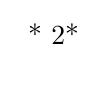
\begin{tikzpicture}
    \addtolength{\boxw}{\boxroundness * 2}
    \addtolength{\boxh}{\boxroundness * 2}

    \foreach \x in {0,.05,...,1}
    {
        \setlength{\tmpa}{\shadowsize * \real{\x}}
        \fill[xshift=\shadowsize - 1pt,yshift=-\shadowsize + 1pt,
                black,opacity=.04,rounded corners=\boxroundness]
            (\tmpa, \tmpa) rectangle +(\boxw - \tmpa - \tmpa,
                \boxh - \tmpa - \tmpa);
    }

    \filldraw[fill=lightorange, draw=black!50, rounded corners=\boxroundness]
        (0, 0) rectangle (\boxw, \boxh);
    \draw node[xshift=\boxroundness,yshift=\boxroundness,
        inner sep=1pt,outer sep=1pt,anchor=south west]
             (0,0) {\usebox{\shadowblockbox}};
\end{tikzpicture}}


%%%%%%%%5

\newcommand{\ceil}[1]{\left\lceil{#1}\right\rceil}

\newcommand{\optimize}[4]{%
  \begin{align}
    \min_{\substack{#2}}\quad & \label{opt:#1} #3 \\
    \text{subj. to}\quad & \nonumber #4
  \end{align}}

\newcommand{\optimizeoneline}[4]{%
  \begin{align}
    \min_{\substack{#2}}\quad & \label{opt:#1} #3 \quad
    \text{subj. to}\quad #4
  \end{align}}

\newcommand{\optimizemax}[4]{%
  \begin{align}
    \max_{\substack{#2}}\quad & \label{opt:#1} #3 \\
    \text{subj. to}\quad & \nonumber #4
  \end{align}}

\newcommand{\optimizemaxoneline}[4]{%
  \begin{align}
    \max_{\substack{#2}}\quad & \label{opt:#1} #3 \quad
    \text{subj. to}\quad #4
  \end{align}}

\newcommand{\optimizeuc}[3]{%
  \begin{align}
    \min_{\substack{#2}}\quad & \label{opt:#1} #3
  \end{align}}

\newcommand{\optimizeLagrange}[4]{%
  \begin{align}
    \max_{\substack{#2}} \min_{\substack{#3}}\quad & \label{opt:#1} #4
  \end{align}}

\newcommand{\optimizemaxuc}[3]{%
  \begin{align}
    \max_{\substack{#2}}\quad & \label{opt:#1} #3
  \end{align}}

\newcommand{\optimizemaxLagrange}[4]{%
  \begin{align}
    \min_{\substack{#2}} \max_{\substack{#3}}\quad & \label{opt:#1} #4
  \end{align}}

%\newtheorem{theorem}{Theorem}
%\newtheorem{definition}{Definitions}

%%% Local Variables: 
%%% mode: latex
%%% TeX-master: "courseml"
%%% End: 

